% intro %
\subsection{Introduction}
When particles collide at high energies inside a particle detector, the collision products either decay into stable particles or simply do not interact with the detector.
In order to identify the original decay products coming out of the collision, we need a way to reconstruct them from the detector signals.
The CMS experiment can achieve this using a holistic approach developed by the ALEPH experiment at LEP called particle flow (PF).

This algorithm uses the various signals captured by the CMS subdetectors, as shown in fig:xxx, %PF_nature_detector),
in order to reconstruct physics objects such as muons, electrons, photons, jets, taus, and missing transverse energy, which are used later in physics analyses.
This section provides a description of the PF algorithm and one of its advanced algorithms for forming energy clusters. Additionally, calorimeter cluster calibration using the conventional method is covered (fix me).

\subsection{Particle Flow Algorithm}
The PF algorithm aims to reconstruct and identify all the final particles produced in an event by utilizing the fact that different particles leave different signatures in the CMS subdetectors, as shown in (fig:). %cms_particle_signtures).
The PF algorithm is used in two different modes in CMS: online PF is used during data collection to select interesting events, and offline PF is utilized after data is collected for offline data analyses. %source for PF and HLT).

The PF algorithm steps as follow. (%source)
First, the PF algorithm reconstructs essential elements: charged particle tracks and energy clusters.
Later in this chapter, the details of the clustering algorithm and the clusters' calibration will be discussed.
Second, it links the PF elements based on their spatial proximity.
The linking rule here is to connect small elements to the bigger ones, meaning they must be touching in the eta-phi space.
The order of the elements is from small to big: track, ECAL cluster, and HCAL cluster.
Examples of links between the elements are: tracks and ECAL clusters, tracks and HCAL clusters, and an inner tracks and muon tracks.
After all the established links, the PF blocks contain groups of linked tracks and clusters.
Any left elements, such as a single track or a cluster,  their own blocks.

Third, a list of PF particle candidates which follows a strict order, starting with the cleanest signature in the CMS muons.
Then, isolated electrons and photons.
After that, neutral hadrons and non-isolated photons.
Lastly, everything left is charged hadrons.
For charged hadrons, the energy is determined by comparing the cluster energy sum to the track momenta sum.
Also, any tracks that are alone are assigned as charge hadrons.

\subsection{Calorimeter Clustering}
The clustering algorithm used in the PF computes the cluster positions and their energies.
This algorithm is done separately in each calorimeter through multiple steps.
First, we identify topological clusters by looking for a group of calorimeter cells with energy deposits above a certain threshold, and they must share at least one neighbor.
The threshold values could be viewed in (fig:).
Next, we identify any calorimeter cell, or seed whose energy is a local maximum with respect to its immediate neighbors so that each topological cluster could have one seed or multiple as shown in (fig:).

Lastly, we compute the cluster positions and energies.
In the single-seed case, the cluster energy will be the sum of all the individual cell energies within the cluster, and its position will be the energy-weighted average of the individual cell positions.
However, for the multiple-seed case, each seed is assumed to represent a unique energy cluster and the energy deposited in non-seed cells will be shared between the various clusters within the topological cluster.
Here the cluster energies and positions will converge using an iterative procedure based on the energy-weighted averages of fractional cell energies. (source)

%------------ figures ------------%
% PF %
\begin{figure}[t!]
\centering
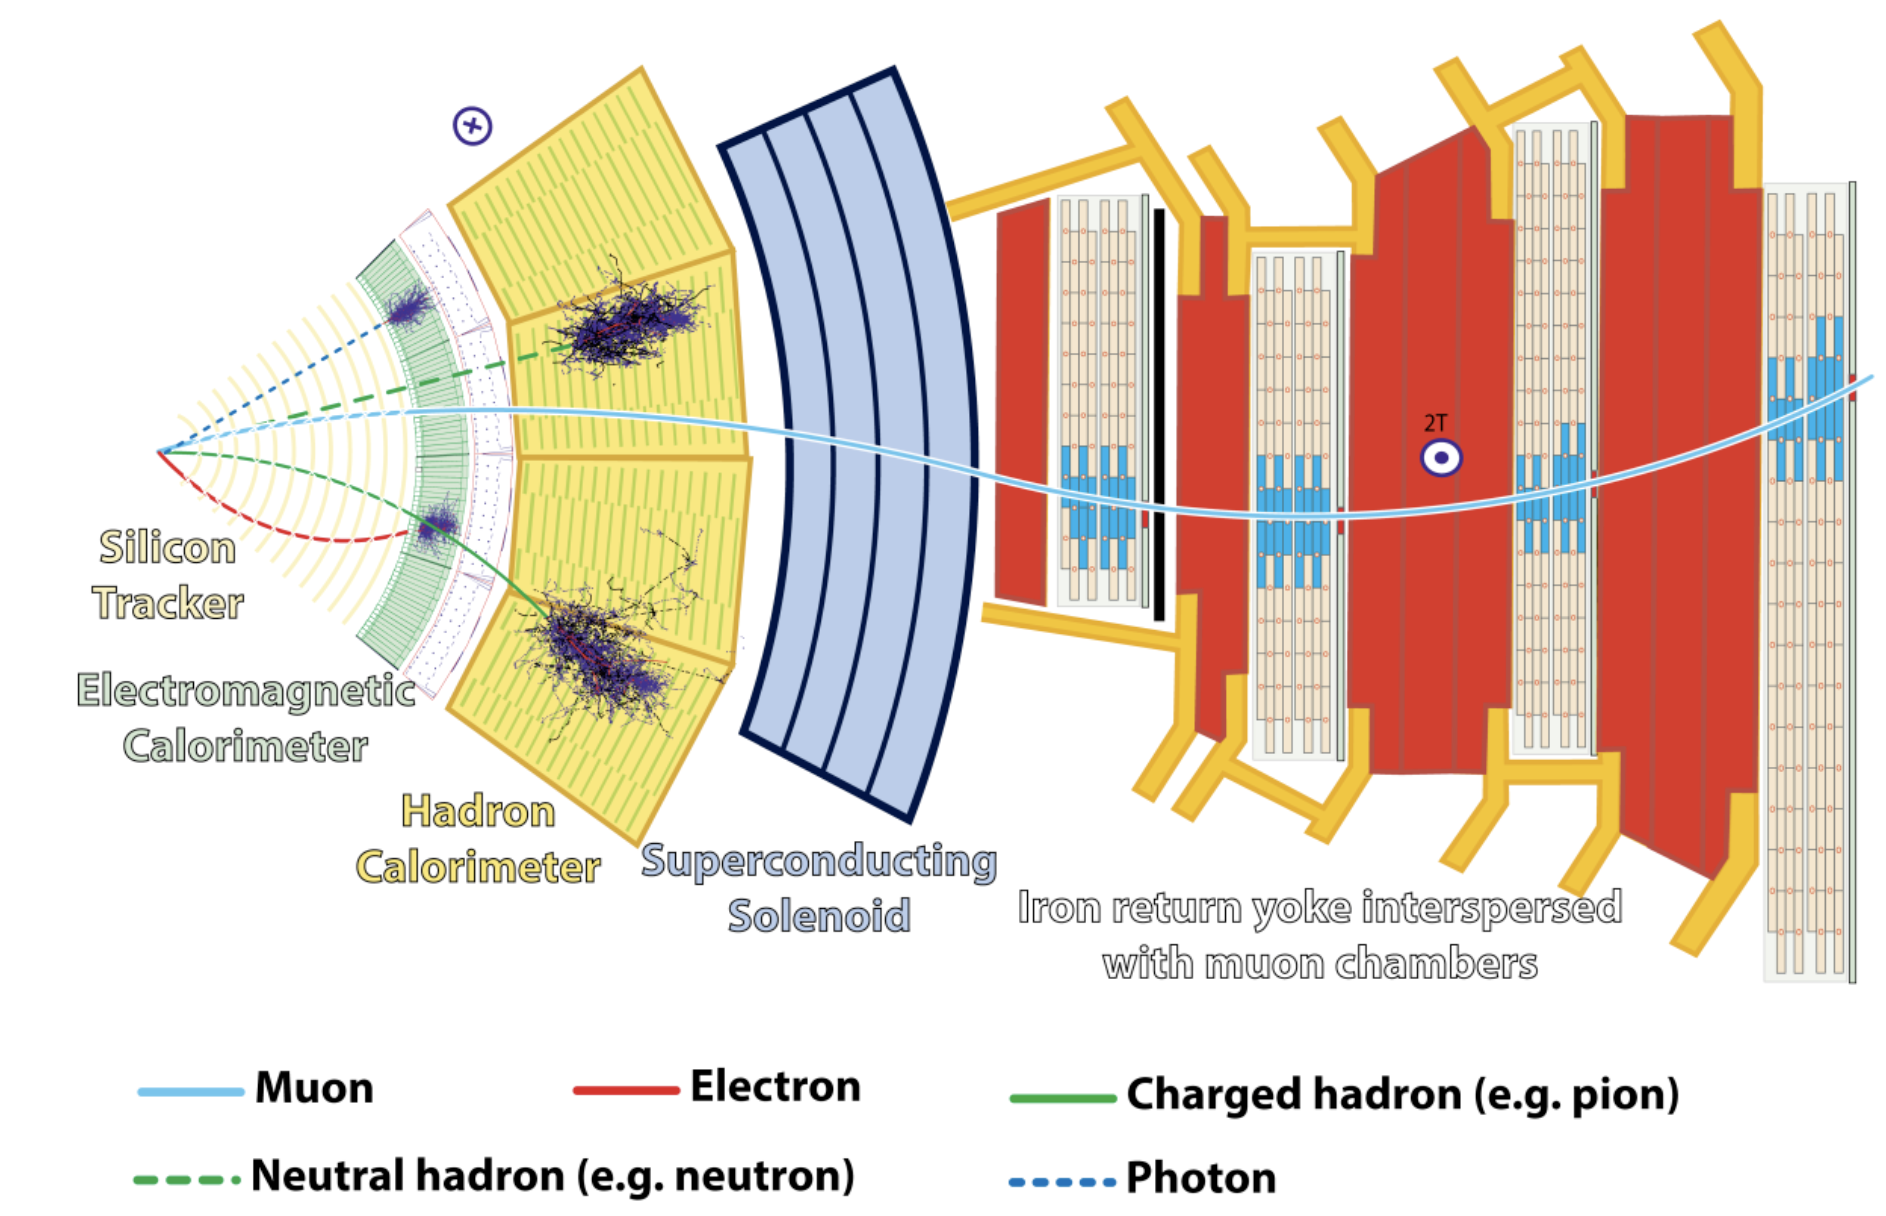
\includegraphics[width=0.99\textwidth]{figures/particles_signture_in_detector.png}
\caption[Particles signture in detector]{Particles signture in detector. Figure source~\cite{}.}
\label{fig:Particles_in_CMS}
\end{figure}

\begin{figure}[t!]
\centering
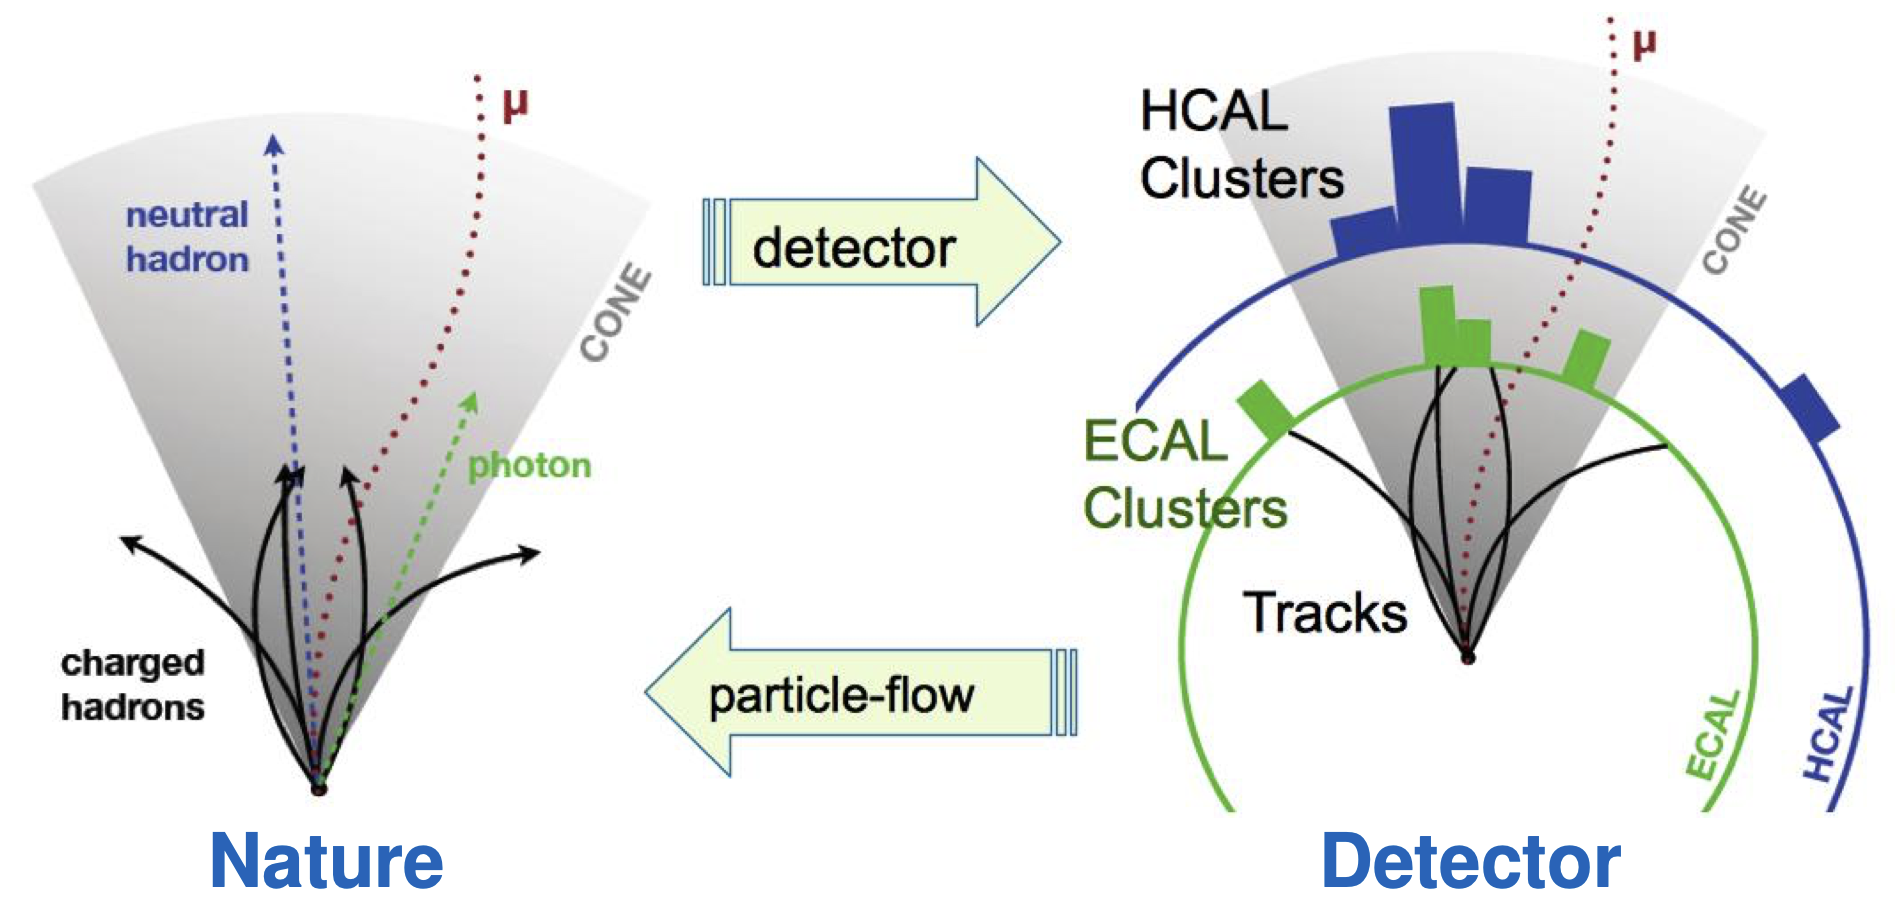
\includegraphics[width=0.99\textwidth]{figures/PF.png}
\caption[PF translate detector information]{PF translate detector information. Figure source~\cite{}.}
\label{fig:PF_diagram}
\end{figure}

% clusering %
\begin{figure}[t!]
\centering
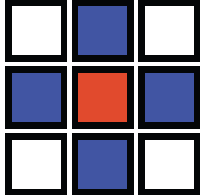
\includegraphics[width=0.25\textwidth]{figures/seed_4neighbours.png}
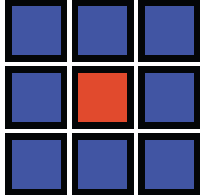
\includegraphics[width=0.25\textwidth]{figures/seed_8neighbours.png}
\caption[Different types of seeds]{Different types of seeds. Figure source~\cite{}.}
\label{fig:seeds}
\end{figure}

\begin{figure}[t!]
\centering
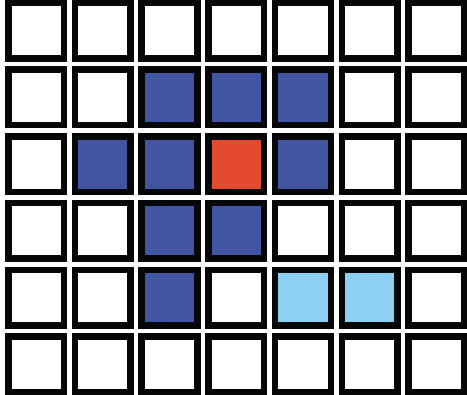
\includegraphics[width=0.25\textwidth]{figures/topological_cluster_oneseed.png}
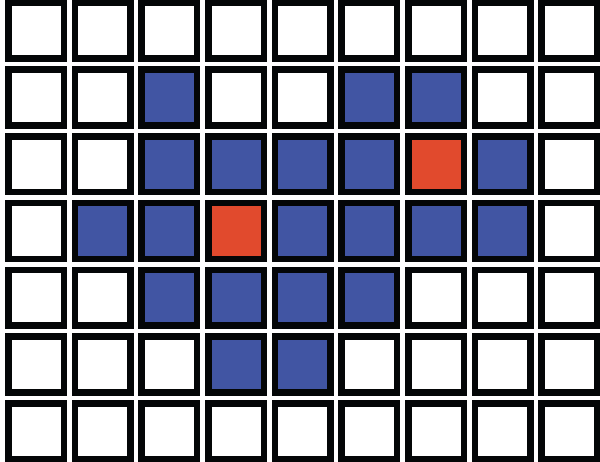
\includegraphics[width=0.25\textwidth]{figures/topological_cluster_many_Seeds.png}
\caption[Types of topological cluster]{Types of topological cluster. Figure source~\cite{}.}
\label{fig:topo_cluster}
\end{figure}

\begin{figure}[t!]
\centering
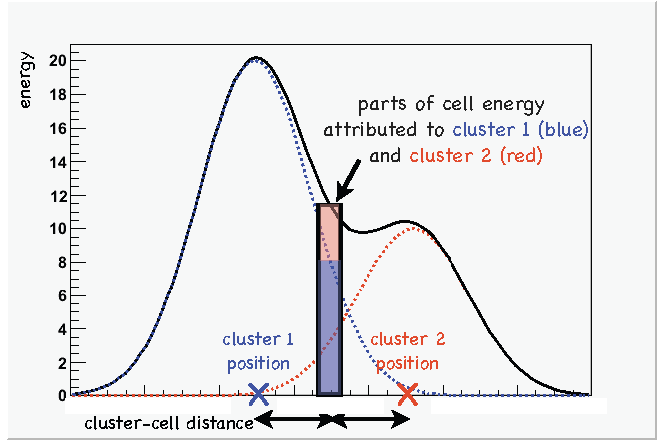
\includegraphics[width=0.50\textwidth]{figures/energy_sharing.png}
\caption[Energy shared between clusters]{Energy shared between clusters. Figure source~\cite{}.}
\label{fig:clustering}
\end{figure}
